\documentclass{article}
\usepackage[utf8]{inputenc}
\usepackage{amssymb,amsmath,graphicx,indentfirst}

\title{EP3 - Método de Monte Carlo}
\author{George Othon\\NUSP 103xxxxx}
\date{April 2020}

\begin{document}

\maketitle

\section{Introdução}

\par
Este relatório tem como objetivo analisar os resultados obtidos pelo Método de Monte Carlo nas suas 4 variações ao integrar f(x) utilizando um gerador de quasi-aleatórios. Para gerar os números Quasi-aleatórios foi empregada a biblioteca ChaosPy.
\[
f(x) = e ^ {-ax} \cos{bx}
\]

Com a = 0.RG e b = 0.NUSP, no intervalo [0,1]. (Com RG = 39xxxxxxx e NUSP = 103xxxxx, logo, a  = 0.39xxxxxxx e b = 103xxxxx ).\\

\section{Bibliotecas}
Para nos axiliar no manuseio das listas, gerar os números aleatórios e para utilzar funções matemáticas e estatísticas que não temos nas built-in do Python, foi necessário importar as seguintes bibliotecas com as seguintes funções:


\begin{enumerate}

    \item Numpy
    
        \begin{enumerate}
        
            \item exp() - Função exponecial 
            \item cos() - Cosseno
            \item std() - Desvio padrão
            \item sqrt() - Raíz quadrada
            \item mean() - Média
            \item cov() - Covariância
            \item var() - Variância
            
        \end{enumerate}
        
    \item ChaosPy
    
        \begin{enumerate}
        
            \item Uniform() - Distribuição uniforme
            \item J() - Joint operator
            \item sample() - Amostra
            \item Beta() -  Distribuição de probabilidade beta
            
        \end{enumerate}
        
    \item Scipy
    
        \begin{enumerate}
        
            \item stats.beta.pdf() - Função de densidade de probabilidade
            
        \end{enumerate}
        
\end{enumerate}

\section{Gerador quasi-aleatório}
A biblioteca ChaosPy foi a escolhida para gerar os números quasi-aleatórios, retornando sempre a mesma lista de números respeitando os requisitos necessários para um gerador quasi-aleatório. Para testar com outros dados geramos a lista de quasi-aleatório e escolhemos um número ao acaso.

\section{Critério de parada}
Como critério de parada utilizamos o erro padrão, onde a cada iteração verificamos se o erro é menor que $1\%
$, e assim que atendesse o critério, ele calcula a média das iterações e retorna como resultado final.


\section{Método Crud}
Este foi o primeiro método que testamos e o mais simples onde apenas calculamos $\frac{1}{n}\sum_{i=1}^n f(x)$, que rendeu bons resultados, e teve desvio padrão de $\sigma = 0.0170$
        

\section{Método Hit or miss}
Ao tentar aproximar a integral de f(x) no intervalo [0,1] geramos diversos pares ordenados (x,y) e verificamos se y $\leq$ f(x), ou seja, se o par ordenado tem imagem acima ou abaixo da função f, e usamos essa proporção para aproximar $\int_0^1 f(x)dx$. Apresentou desvio padrão $\sigma = 0.0100$ 

\section{Método Importance Sampling}
No método em questão, utilizamos um gerador de números pseudo-aleatórios com distribuição beta. Após diversos testes tivemos os melhores resultados com os parâmetros $ \alpha = 0.9 $ e $ \beta = 1.0 $. Nessas condições tivemos boas aproximações, e com diversos testes o desvio padrão foi de $ \sigma = 0.0046$

\section{Método Control Variate}
No Control Variate, após algumas análises escolhemos como aproximação para f(x), a função $ g(x) = e ^ {-ax}$, com a = 0.399104525. Como $ g(x) > f(x), \; \forall x \in [0,1] $, e g(x) é extremamente próxima à f(x).
\par
Dividimos este método em duas partes. Na primeira calculamos o resultado da integral pelo método Crud para f(x) e para g(x). Na segunda parte, calculamos o fator \textbf{c} dado por $$c = \frac{-Cov[f(x),g(x)]}{Var[g(x)]}$$ e em seguida calculamos $$Crud(f(x)) + c * (Crud(g(x) - \int_0^1 g(x) dx )$$ onde $\int_0^1 g(x) dx = 0.824$, para obter a aproximação final, que teve excelentes resultados apresentando desvio padrão $\sigma = 0.0007$

\section{Comparando os métodos}

Rodamos cada método 100 vezes e fizemos o seguinte resumo estatístico com o auxílio da biblioteca pandas. 
\par 
Utilizamos o jupiter notebook para gerar a tabela a seguir, e incluimos como uma imagem no artigo. Para a criação da tabela foram usadas as funções DataFrame() e describe().

\hfill

%Tabela (imagem) análise descritiva

\begin{figure}[!htb]
    \centering
    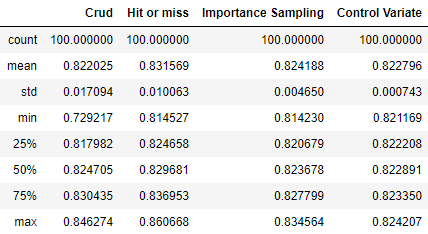
\includegraphics[scale=0.7]{Descritiva Quasi.PNG}
    \caption{Análise Descritiva ( n = 100 )}
    \label{fig:my_label}
\end{figure}

\hfill

\par
Ao análisar a tabela acima percebemos que para todos os métodos a média e a mediana ( 50\% ) fica próximo à 0.82. O método Crud foi o que teve a maior variação e o Control Variate teve a menor. Mas escolhemos o desvio padrão para analisar o desempenho de cada método, e com base nesse parametro fizemos a seguinte classificação dos métodos.

\hfill

% Tabela de classificação dos métodos

\begin{table}[ht]
    \centering
    \begin{tabular}{c|c|c}
         & Método & Desvio padrão \\
         \hline
        1 & Control Variate & 0.0007 \\
        \hline
        2 & Importance Sampling & 0.0046 \\
        \hline
        3 & Hit or miss & 0.0100 \\
        \hline
        4 & Crud & 0.0170 \\
        
    \end{tabular}
    \caption{Classificação dos métodos}
    \label{tab:my_label}
\end{table}

\hfill

\par 
Portanto, dentre os quatro métodos que implementamos, o que retornou os melhores resultados foi o Método Control Variate utilizando a função g como aproximação para f.


\subsection{Comparando os geradores}
Ao comparar as aproximações com os geradores pseudo e quasi-aleatórios tivemos melhor resultados com o gerador quasi, exceto no método Control Variate que foi o melhor dos métodos com utilizando o gerador de pseudo-aleatório. Classificamos os métodos com cada gerador pelo desvio padrão apresentado e obtivemos a seguinte tabela.

\hfill

%Tabela comparando os métodos e geradores

\begin{table}[ht]
    \centering
    \begin{tabular}{c|c|c|c}
         & Método & Gerador & Desvio padrão \\
        \hline
        1 & Control Variate & Pseudo & 0.0006 \\
        \hline
        2 & Control Variate & Quasi & 0.0007 \\
        \hline
        3 & Importance Sampling & Quasi & 0.0046 \\
        \hline
        4 & Importance Sampling & Pseudo & 0.0048 \\
        \hline
        5 & Hit or miss & Quasi & 0.0100 \\
        \hline
        6 & Hit or miss & Pseudo & 0.0108 \\
        \hline
        7 & Crud & Quasi & 0.0170 \\
        \hline
        8 & Crud & Pseudo & 0.0203 \\
        
    \end{tabular}
    \caption{Comparação métodos e geradores}
    \label{tab:my_label}
\end{table}

Desse modo, para uma melhor aproximação para a nossa integral no intervalo [0,1] utilizamos o método Control Variate, que nos proporcionou as duas melhores aproximações alterando entre os geradores pseudo e quasi-aleatório, e apesar da pequena diferença, tivemos melhores resultados quando usamos o gerador pseudo-aleatório.


%Referências bibliográficas 

\begin{thebibliography}{4}

\bibitem{NumPy}
https://numpy.org/doc/
\bibitem{ChaosPy}
https://chaospy.readthedocs.io/en/master/tutorial.html
\bibitem{SciPy}
https://docs.scipy.org/doc/scipy/reference/stats.html
\bibitem{Livro}
Cognitive Constructivism and the Epistemic Significance of Sharp Statistical Hypotheses in Natural Sciences - Julio Stern

\end{thebibliography}

    
\end{document}
